\documentclass[border=2pt,convert]{standalone}

\usepackage{pgfplots}
\pgfplotsset{compat=1.17}

\begin{document}

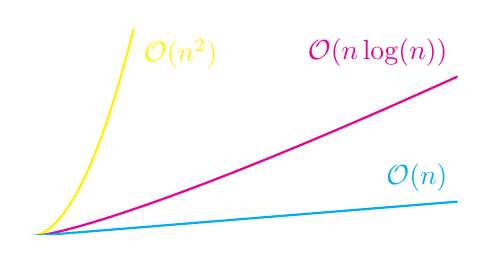
\begin{tikzpicture}
    \begin{axis}[
        width=200,
        height=120,
        ticks=none,
        axis x line=middle,
        axis y line=middle,
        domain=0:100,
        restrict y to domain=0:600,
        samples=500,
        no markers,
        thick,
        white,
        axis on top=true,
        ]
        \addplot+[yellow]  {x^2}     node[below right] {$\mathcal O(n^2)$};
        \addplot+[magenta] {x*ln(x)} node[above left]  {$\mathcal O(n\log(n))$};
        \addplot+[cyan]    {x}       node[above left]  {$\mathcal O(n)$};
    \end{axis}
\end{tikzpicture}

\end{document}
